\chapter{The DLS Method in Detail}

We now look at the mathematics behind the D/L, and DLS methods. D/L being the original
method, and DLS the method that Stern helped to revise. In the original paper, the authors
state ``Commercial confidentiality prevents the disclosure of the mathematical definitions
of these functions.'' $\cite{duckworth}$. Which is naturally a slight problem for this, but what
we can do is instead use sample values based on data we have to look at how these functions behave,
so all is certainly not lost.

\section{Origins: Duckworth and Lewis}
We begin by looking at the original paper. The first thing to establish is how many runs are scored,
on average, in a given number of overs. This is given by the equation:

\begin{equation}
    Z(u) = Z_0[1-exp(-bu)]
    \label{Z(u)}  
\end{equation}

Where u is the number of overs, b is the exponential decay constant, and $Z_0$ is the
average total score in first class cricket, but with one-day rules imposed.  

Now because we don't have access to actual values for $Z_0$ or b, a plot to see what equation \ref{Z(u)} looks 
like was created by using 3 sample values for $Z_0$. For b, it was a process of trial and error to find a value
that resulted in the graph having a similar shape to original figures in the D/L paper. 

\begin{figure}[h]
    \centering
    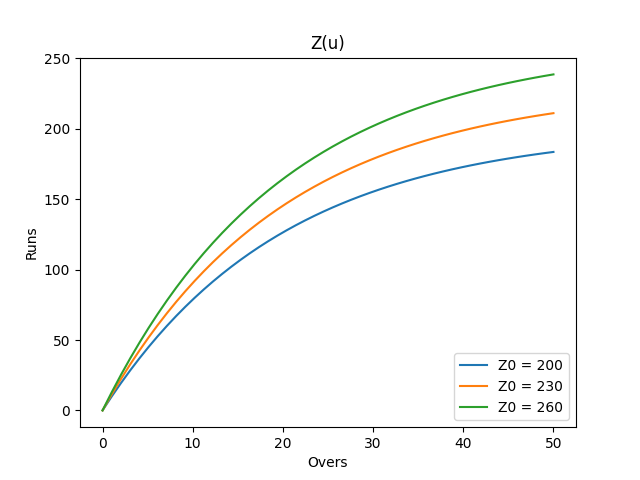
\includegraphics[scale=0.6]{figures/z(u).png}
    \label{Z(u)_graph}
\end{figure}

However, we have not yet looked at what happens when wickets are lost. To introduce this metric, equation \ref{Z(u)}
is revised to incorperate the scenario that w wickets have been lost, and that there are u overs remaining
The revised equation is given as follows:

\begin{equation}
    Z(u,w) = Z_0(w)[1-exp(-b(w)u)]
    \label{zuw}
\end{equation}

Where now, we have $Z_0(w)$ giving the average total score from the last $10-w$ wickets in first class cricket.
We now also have $b(w)$ as the exponential decay constant, which now changes depending on wickets lost.

%Should probably make a plot of this, to go with the other one, but due to confientiality
%it's quite hard to get the numbers for Z0(u,w) myself.

With this in mind, we now look at the specific case of equation \ref{zuw} with $u=N$ and $w=0$, namely, the conditions
at the start of an N-over innings. We have:

\begin{equation}
    Z(N,0) = Z_0[1-exp(-bN)].
    \label{zstart}
\end{equation}

Which we then incorperate into the ratio

\begin{equation}
    P(u,w) = \frac{Z(u,w)}{Z(N,0)}.
    \label{prat}
\end{equation}

The ratio \ref{prat} gives, keeping in mind there are u overs still to be bowled, with w wickets
lost, the average proportion of the runs that still need to be scored in the innings. 
It is this ratio that is where the revised scores come from. Let us now look a bit more at how that works
practically.

\begin{example}
    \label{dlExMain}
    Assume there is a break in the second innings (due to rain or similar), which results in the second team missing some overs.
    Let $u_1, u_2$ be the number of overs played before the break, and available after it respectively. We impose the condition
    that $u_2 < u_1$. At the time of the break, the second team had lost $w$ wickets. The aim is to adjst the required score to account
    for the $u_1 - u_2$ overs they have lost. The winning ``resources'' available are given by

    \[
        R_2 = [1-P(u_1,w)+P(u_2,w)].
    \]  

    Which means, if the first team batting scored S runs, then the new tartget is given by

    \[
        T = \ceil{SR_2}
    \]  
\end{example}

\section{Improvements by Stern}
foo